\documentclass[a0paper,landscape]{baposter}

\usepackage{multicol} % For handling multiple columns
\usepackage{lipsum} % For sample text
\usepackage{tikz}
\usepackage{graphicx}
\usepackage{caption}
\usepackage{hyperref}

\usepackage{enumitem}
\setlist{nosep} % Removes extra spacing between items and around the list

\usepackage[final,protrusion=true,expansion=true]{microtype} % nice font tweaks
\usepackage[small,compact, sf]{titlesec} % reduce space
%\usepackage[margin=1in]{geometry} % set page margins automatically 
%% \usepackage[parfill]{parskip}  % paragraphs have vert space not indent
\usepackage[sc]{mathpazo} % Palatino font


%% \usepackage[backend=bibtex,style=numeric]{biblatex} % Load biblatex
%% \addbibresource{library.bib} % Replace with your .bib file name

\renewcommand*{\bibfont}{\footnotesize} % footnotesize scriptsize tiny

%\usepackage[bibstyle=authoryear,giveninits=true,maxbibnames=99]{biblatex}
\usepackage[hyperref=true,
            %sorting=none, 
            sorting=nyt,
            %style=numeric, 
            date=year,
            style=authoryear,
            %defernumbers=true, 
            firstinits=true, 
            uniquename=false,
            uniquelist=false,
            %uniquelist=minyear,
            maxnames=99, 
            maxcitenames=1]{biblatex}
\renewbibmacro{in:}{}

\addbibresource{library.bib}
%% addbibresource{/path/to/library.bib}
%% biber <texfile><.NOEXT> --output_format bibtex
%% biber --output_format=bibtex --output_resolve ${fn}.bcf

% Don't print URL if DOI field exists
\DeclareFieldFormat{url}{%
  \iffieldundef{doi}{%
    \mkbibacro{URL}\addcolon\space\url{#1}%
  }{%
  }%
}
% Don't print URL if DOI field exists
\DeclareFieldFormat{urldate}{%
  \iffieldundef{doi}{%
    \mkbibparens{\bibstring{urlseen}\space#1}%
  }{%
  }%
}

\renewbibmacro*{journal+issuetitle}{%
  \usebibmacro{journal}%
  \setunit*{\addspace}%
  \iffieldundef{series}
               {}
               {\newunit
                 \printfield{series}%
                 \setunit{\addspace}}%
               \usebibmacro{issue+date}%
               \setunit{\addcomma\space}%
               \usebibmacro{volume+number+eid}%
               \setunit{\addcolon\space}%
               \usebibmacro{issue}%
               \newunit}

\newbibmacro*{issue+date}{%
  \iffieldundef{issue}
               {. \usebibmacro{date}}
               {\printfield{issue}%
                 \setunit*{\addspace}%
                 \usebibmacro{date}}%
               \newunit}

\renewbibmacro*{volume+number+eid}{%
  \printfield{volume}%
  \setunit*{\addnbspace}% NEW (optional); there's also #+LATEX_HEADER_EXTRA: \addnbthinspace
  \printfield{number}%
  \setunit{\addcomma\space}%
  \printfield{eid}}
\DeclareFieldFormat[article]{number}{\mkbibparens{#1}}
\DeclareFieldFormat{pages}{#1}

\setlength{\bibitemsep}{0.33\baselineskip} % Add space between items
\setlength{\bibhang}{0pt} % Remove indentation


\begin{document}

\definecolor{NASAblue}{rgb}{0.04,0.24,0.57} % NASA meatball blue
\definecolor{NASAred}{rgb}{0.99,0.24,0.13} % NASA meatball red

\begin{poster}%
  % Poster Options
  {
    columns=10,
    % Show grid to help with alignment
    grid=true,
    % Column spacing
    colspacing=1em,
    % Color style
    bgColorOne=white,
    bgColorTwo=black,
    borderColor=NASAred,
    headerColorOne=NASAblue,
    headerColorTwo=NASAblue,
    headerFontColor=white,
    boxColorOne=green,
    boxColorTwo=cyan,
    % Format of textbox
    textborder=faded,
    % Format of text header
    eyecatcher=true,
    headerborder=closed,
    headerheight=0.13\textheight,
    %  textfont=\sc, An example of changing the text font
    headershape=roundedright,
    headershade=shadelr,
    headerfont=\Large\bf\textsc, %Sans Serif
    textfont={\setlength{\parindent}{0em}\setlength{\parskip}{1ex}},
    boxshade=plain,
    %  background=shade-tb,
    background=plain,
    linewidth=2pt
  }
  { % top left graphic
    
\includegraphics[height=3cm]{fig/NASA.png}
    %% \begin{minipage}{0.1\textwidth}
    %%   \centering 
    %%   \Large Poster \#\\
    %%   Some Number Or Figure
    %% \end{minipage}
  }
  { % title
    \bfseries{Title of\\the Poster}
  }
  { % authors
  \begin{minipage}[t]{0.9\textwidth}
    \centering {\normalsize
      \renewcommand{\baselinestretch}{1.0}\selectfont
      \vspace{1ex}
      Some A. Author, Another B. Person
    }
  \end{minipage}
  }
  { % top right graphic
    
\includegraphics[height=3cm]{fig/NASA.png}
    %% \includegraphics[height=3cm]{fig/modelE.png}
  }


  

\headerbox{Introduction}{name=introduction,column=0,span=5}  {
This README.org file implements \texttt{org\_baposter}. The results can be seen in README.pdf. It's not a well-developed package (pull requests accepted) but works for me. This README should help you get things working if you prefer to use \texttt{Org Mode} instead of \LaTeX{} for your poster development.

\texttt{baposter} support is not yet a full \texttt{Emacs} package accessible entirely through \texttt{Org Mode}. This \texttt{org\_baposter} setup requires editing some \LaTeX{} code.

\textbf{Org Baposter}

\texttt{Org Mode} support for \texttt{baposter} is implemented by the code block at the bottom of this file. Evaluate it, then export this file with \texttt{C-c C-e p p}, then compile the generated \texttt{.tex} file.

\textbf{Poster Header}

The poster header (logos, title, authors) and style (box shapes, colors, etc.) are maintained in \LaTeX{}. Edit \texttt{org\_baposter.tex} directly. The background grid can be turned off by setting \texttt{grid} to \texttt{false} or commenting out \texttt{grid=true}.

\textbf{References}

References are placed in \texttt{library.bib} and controlled by \texttt{references.tex}. At the moment all references are included via a \texttt{\textbackslash{}nocite\{*\}} but this can be changed.

}
\headerbox{Tables}{name=tables,column=5,span=5}  {
There is limited support for \texttt{Org Babel}. Tables must be embedded in a \texttt{:results drawer}.

\phantomsection
\label{}
\begin{center}
\begin{tabular}{lrrr}
 & foo & bar & baz\\
\hline
a & 5.851 & 3.701 & 4.677\\
b & 7.526 & 5.137 & 6.964\\
c & 7.935 & 3.939 & 4.827\\
\end{tabular}
\end{center}

}
\headerbox{Figures}{name=figures,column=5,span=5,below=tables}  {
There is limited support for \texttt{Org Babel}. As with tables, figures generated by \texttt{Org Babel} can be wrapped in a \texttt{drawer}, but \texttt{\#+CAPTION} and sizing (via \texttt{\#+ATTR\_LATEX}) are not supported. It is easier to generate the figure with \texttt{:exports none} and then use raw \LaTeX{} code to include it. 

\begin{center}
  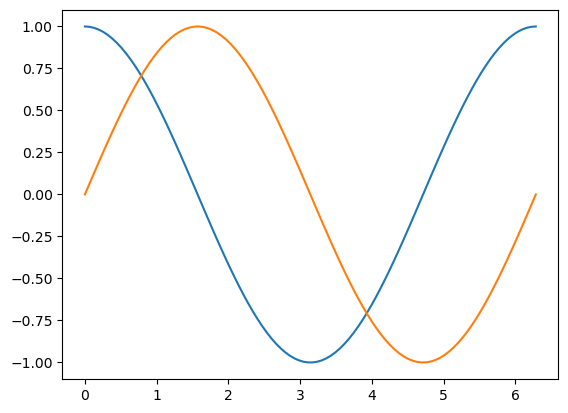
\includegraphics[width=0.45\linewidth]{fig/fig.png}
  \captionof{figure}{\label{fig:some_fig}This figure is generated with the code above. Neither the code or figure are exported. The figure is then placed with LaTeX code.}
\end{center}

}
\headerbox{Lists and Text}{name=lists-and-text,column=0,span=5,below=introduction}  {
Normal \texttt{Org Mode} syntax is supported including \textbf{bold} and \emph{italic}, and other features.

\begin{itemize}
\item Lists (but without checkboxes)
\item Sub-lists
\begin{itemize}
\item Item 1
\item Item 2
\end{itemize}
\end{itemize}

And if you prefer, you can embed \LaTeX{} anywhere you like.

\vspace{7mm}

}
\headerbox{Lorem}{name=lorem,column=0,span=3,below=lists-and-text}  {
\lipsum[1][1]

\lipsum[1][2]

\lipsum[1][3-4]

}
\headerbox{Ipsum}{name=ipsum,column=3,span=7,below=figures}  {
\begin{multicols}{2}
\lipsum[2]
\end{multicols}

}
\headerbox{References}{name=references,column=0,span=10,above=bottom}  {
\begin{multicols}{3}
  \nocite{*}
  \printbibliography[heading=none]
\end{multicols}

}

\end{poster}
\end{document}
